% VLDB template version of 2020-03-05 enhances the ACM template, version 1.7.0:
% https://www.acm.org/publications/proceedings-template
% The ACM Latex guide provides further information about the ACM template

\documentclass{article}
\usepackage{listings}
\usepackage[margin=20mm]{geometry}
\usepackage{graphicx}
\usepackage{amsfonts}
\usepackage{amsmath}
\usepackage{physics}
\usepackage{parskip}
\usepackage{enumitem}
\usepackage{cancel}

%% The following content must be adapted for the final version
% paper-specific
\newcommand\vldbdoi{XX.XX/XXX.XX}
\newcommand\vldbpages{XXX-XXX}
% issue-specific
\newcommand\vldbvolume{14}
\newcommand\vldbissue{1}
\newcommand\vldbyear{2020}
% should be fine as it is
\newcommand\vldbauthors{\authors}
\newcommand\vldbtitle{\shorttitle} 
% leave empty if no availability url should be set
\newcommand\vldbavailabilityurl{http://vldb.org/pvldb/format_vol14.html}
\newcommand\oname{\operatorname}

\newtheorem{theorem}{Teor.}
\newtheorem{definition}{Def.}
\newtheorem{example}{Ej.}
\newtheorem{excercise}{Ejer.}

\begin{document}

\textbf{Ex. 3.1: }Why isn't the multiplicity factor $(3-16)$ just $n!$? After all, we started this discussion by stipulating that the balls, in addition to having colors, also carry labels $(1\cdots N)$, so that different permutations of the red balls among themselves, which give the $r!$ in the denominator of $(3-16)$, are distinguishable arrangements.

\textbf{Answer: }

We've decomposed the event ``drawing $r$ red balls in $n$ draws'' as the union of events of the form ``draw $r$ red balls in $n$ draws with the particular permutation of orders $p$'' for permutations $p$, which are mutually exclusive and identically plausible. At doing this, we're using the events $R_i$ and $W_i$, with the probability given by $(3-14)$. If we were to use ``drawing the following $n$ balls, where $r$ are red'', we should be accounting for the probability $B_{ij}$ of drawing the $i$th ball after $j$ draws, which would incorporate the missing factors.

\textbf{Ex. 3.2: Probability of a Full Set: }Suppose an urn contains $N=\sum_iN_i$ balls, $N_1$ of color $1$, $N_2$ of color $2$, $\cdots$, $N_k$ of color $k$. We draw $m$ balls without replacement; what is the probability that we have at least one of each color? Supposing $k=5$, all $N_i=10$, how many do we need to draw in order to have at least $90\%$ probability of getting a full set?

\textbf{Answer: }

We're asked $P\left(\sum_{r\in I}\prod_ir_i\right)$, where $I=\{(r_i):\,r_i\geq1\forall i\}$. We can decompose this as 
\begin{align}
	P\left(\sum_{r\in I}\prod_ir_i|B\right)&=\sum_{r\in I}P\left(r_1\cdots r_k|B\right)\\
	&=\frac1{\begin{pmatrix}N\\m\end{pmatrix}}\sum_{r\in I}\prod_i\begin{pmatrix}N_i\\r_i\end{pmatrix}
\end{align}

A calculation is probably better done by calculating the missing terms instead, which are those for which at least one of those are $0$, of which there are less, since at least one of the summands is already $0$, the rest varying between the same intervals.

The ``3.2.py'' script does the maths, and outputs $m=15$ as the solution, with a probability of about $0.91$.

\textbf{Ex. 3.3: Reasoning Backwards: }Suppose that in the previous exercise $k$ is initially unknown, but we know that the urn contains exactly $50$ balls. Drawing out $20$ of them, we find $3$ different colors; now what do we know about $k$? We know from deductive reasoning (i.e., with certainty) that $3\leq k\leq 33$; but can you set narrower limits $k_1\leq k\leq k_2$ within which it is highly likely to be?

\textbf{Answer:}

I suppose this is the first use case of Bayes theorem as it's usually used. By letting the hypotheses $H_k=\text{``There are $k$ different colors in the urn''}$ and the data $D=\text{``3 different colors have been seen after 20 draws''}$, we want $P(H_k|D)$, but what our model tells us with certainty is $P(D|H_k)$, so we'll use Bayes' theorem for this:
\begin{align}
	P(H_k|D)&=\frac{P(D|H_k)P(H_k)}{\sum_kP(D|H_k)P(H_k)}.
\end{align}
I will assume each $H_k$ is equally likely, since I've got no information on anything. Thus,
\begin{align}
	P(H_k|D)&=\frac{P(D|H_k)}{\sum_kP(D|H_k)}.
\end{align}

We're now left with the task of finding the probability that $3$ different colors are seen in a set of $20$ taken from $50$, given there are $k$ different colors. To this end, we split $D=\sum_NDH_N$, where $N\in\mathbb N^k$ is such that $N_i$ is the number of balls with the $i$th color, and get
\begin{align}
	P(D|H_k)&=P\left(\sum_NDH_N\middle|H_k\right)\\
	&=\sum_NP(DH_N|H_k)\\
	&=\sum_NP(D|H_NH_k)P(H_N|H_k).
\end{align}
We once again propose an homogeneous distribution over the $N$, which gives $P(H_N|H_k)=\begin{pmatrix}50-k\\k-1\end{pmatrix}^{-1}$.

Now, let's think of the probability of drawing from only the colors $1$, $2$, and $3$ in all draws. For the $m$th draw, the probability is
\begin{align}
	\frac{51-m-\sum_{l=3}^{k-2}N_l}{51-m}&=\frac{51-m-N_\text{rem}}{51-m},
\end{align}
so for the 20 draws, we get
\begin{align}
	\frac{\left(50-N_\text{rem}\right)!\;30!}{\left(30-N_\text{rem}\right)!\;50!}.
\end{align}

So, the chances of drawing only the first $3$ colors are the sum over all of the $N$ of this term. For each choice of $N_\text{rem}$, there are $\begin{pmatrix}47-N_\text{rem}\\2\end{pmatrix}=(47-N_\text{rem})(46-N_\text{rem})$ such terms. And, by simmetry of label permutation, for each choice of $3$ colors the result is the same, so finally, by splitting $D$ into the sum of ``drawing only for these $3$ particular colors'', we sum over these $k!/(k-3)!$ choices, and get our final result:
\begin{align}
	P(D|H_k)&=\frac{k!}{(k-3)!}\sum_{N_\text{rem}=k-3}^{47}(47-N_\text{rem})(46-N_\text{rem})\frac{(50-N_\text{rem})!\;30!}{(30-N_\text{rem})!\;50!}\begin{pmatrix}50-k\\k-1\end{pmatrix}^{-1}
\end{align}

The ``3.3.py'' script implements this solution, giving the probability distribution shown in Figure \ref{fig:3.3}
\begin{figure}[h]
	\center
	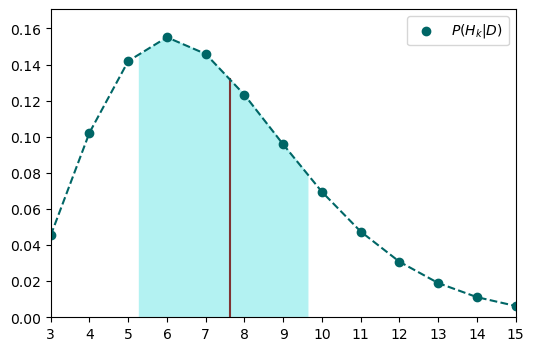
\includegraphics[width=0.5\textwidth]{Numerical/3.3.png}
	\caption{Probability distribution $P(H_k|D)$ for different values of $k$. The shaded region goes between first and third quartile, and the vertical line denotes the (linearly extrapolated) median.}
	\label{fig:3.3}
\end{figure}

\textbf{Ex. 3.4: Matching: }The $M$ urns are now numbered $1$ to $M$, and $M$ balls, also numbered $1$ to $M$, are thrown into them, one in each urn. If the numbers of a ball and its urn are the same, we have a match. Show that the probability of at least one match is
\begin{align*}
	P&=\sum_{k=1}^M(-1)^{k+1}/k!.
\end{align*}

As $M\rightarrow\infty$, this converges to $1-1/e=0.632$. The result is surprising to many, because however large $M$ is, there remains an appreciable probability of no match at all.

\textbf{Answer:}

I give up. The problem turns out to be that of counting derangements, which Wikipedia explains:

Let the urn $1$ receive ball $i$. If urn $i$ receives ball $1$, then we're left with the problem of counting derangements for $M-2$.
If urn $i$ receives a ball other than $1$, then it's the problem of counting derangements for $M-1$, since for each of the other urns there is $1$ ball they may not receive (urn $i$ shall not receive ball $1$). Thus,
\begin{align}
	!n&=(n-1)(!(n-1)+!(n-2)),
\end{align}
which may now be solved by induction.

\textbf{Ex. 3.5: Occupancy: }$N$ balls are tossed into $M$ urns; there are evidently $M^N$ ways this can be done. If the robot considers them all equally likely, what is its probability that each urn receives at least one ball?

\textbf{Answer: }

If they're equally likely, we can just count. We'll count the negative, summing over the number $k$ of boxes with no matches. There are $\begin{pmatrix}M\\k\end{pmatrix}$ such choices, and the rest of boxes allow for $(M-k)^N$ choices, so there are
\begin{align}
	\sum_{k=1}^M\begin{pmatrix}M\\k\end{pmatrix}(M-k)^N
\end{align}
instances where no box receives balls, and thus
\begin{align}
	P(\text{``Each urn receives at least one ball''})&=1-\sum_{k=1}^M\begin{pmatrix}M\\k\end{pmatrix}\left(1-\frac{k}{M}\right)^N
\end{align}

\end{document}
\endinput
